\documentclass{cw1}
\usepackage[T2A]{fontenc}
\usepackage[utf8]{inputenc}
\usepackage[russian]{babel}
\usepackage{multirow}
\usepackage{textcomp}
\usepackage{tikz}
\usepackage{graphicx}

\begin{document}
\sloppy

\title{Модель боя противотанкового резерва ПТУР с контратакующим противником
для разнотипных боевых единиц}

\author{Блабла}
\university{Санкт-Петербургский государственный университет}
\facility{Факультет военного обучения}
\group{642}
\position{студента}
\chair{Кафедра информатики}
\leaderPosition{к.ф.-м.н.}
\leader{блабла}
\city{Санкт-Петербург}
\yr{2011}

\maketitle
\setcounter{page}{2}

\section{Окно настроек}
\begin{center}
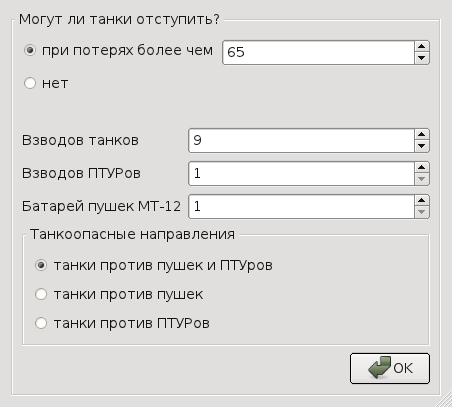
\includegraphics[height=70mm]{img1.png}
\end{center}
Присутствуют следующие настройки модели боя.
\begin{itemize}
 \item Танки отступят при потере указанного (в процентах) количества личного состава.
 \item Танки не отсупают.
 \item Количество взводов танков: от 1 до трех, по 18 танков во взводе.
 \item Количество подразделений ПТУРов от 1 до 2, по трое ПТУР в одном отделении
 \item Количество подразделений гаубиц Д-30. Одна или две батареи
 \item Танкоопасные направления
   \begin{itemize}
    \item Танки против ПТУРов и гаубиц
    \item Танки против гаубиц
    \item Танки против ПТУРов
   \end{itemize}
\end{itemize}


\section{Моделирование}
Моделирование происходит следующим образом, в зависимости от расположения подразделений на танкоопасных направлениях 
реализуется одна из следующих ситуаций:


1) На то танкоопасное направление, по которому пошли танки выставлено несколько подразделений ПТУРов. Тогда, танки 
сначала ведут бой с подразделением ПТУР, потом двигаются до расстояния дальности полёта танкового снаряда (10 км). 
Во время этого марша они оказываются под огнём батарей адн Д-30. Как только танки доходят до рубежей первоначально 
занятых ПТУРами они открывают огонь по арт. батарее. Если танки могут отступать при некоторых потерях, то они 
отступают, в противном случае бой продолжается до полного уничтожения одной из сторон.


2) Танкоопасное направление, куда вышли танки, оказалось не прикрыто подразделением ПТУР. Поэтому танки практически 
сразу оказываются под огнём артилерийских батарей. Подразделения танков продвидаются до рубежа открытия огня и начинают 
бой с батареями. 


3) Танкоопасное направление прикрытое ПТУР, атакуется танками. Завязывается бой. Если танки могут отступить, то в 
зависимости от численности ПТУР они либо отступают, либо уничтожают ПТУР. 

В ходе боя танки делают 2 выстрела в минуту и попадают с вероятностью 0.25. ПТУР делают 2 выстрела в минуту и попадают
 с вероятностью 0.95, а Д-30 делают 4 выстрела в минуту попадая с вероятностью 0.33
Танки перемешаются со скоростью 50 км/ч и преодолевают под огнём батареи адн не менее 5 км.

Моделирование поля боя представлено на следующей иллюстрации:

\begin{center}
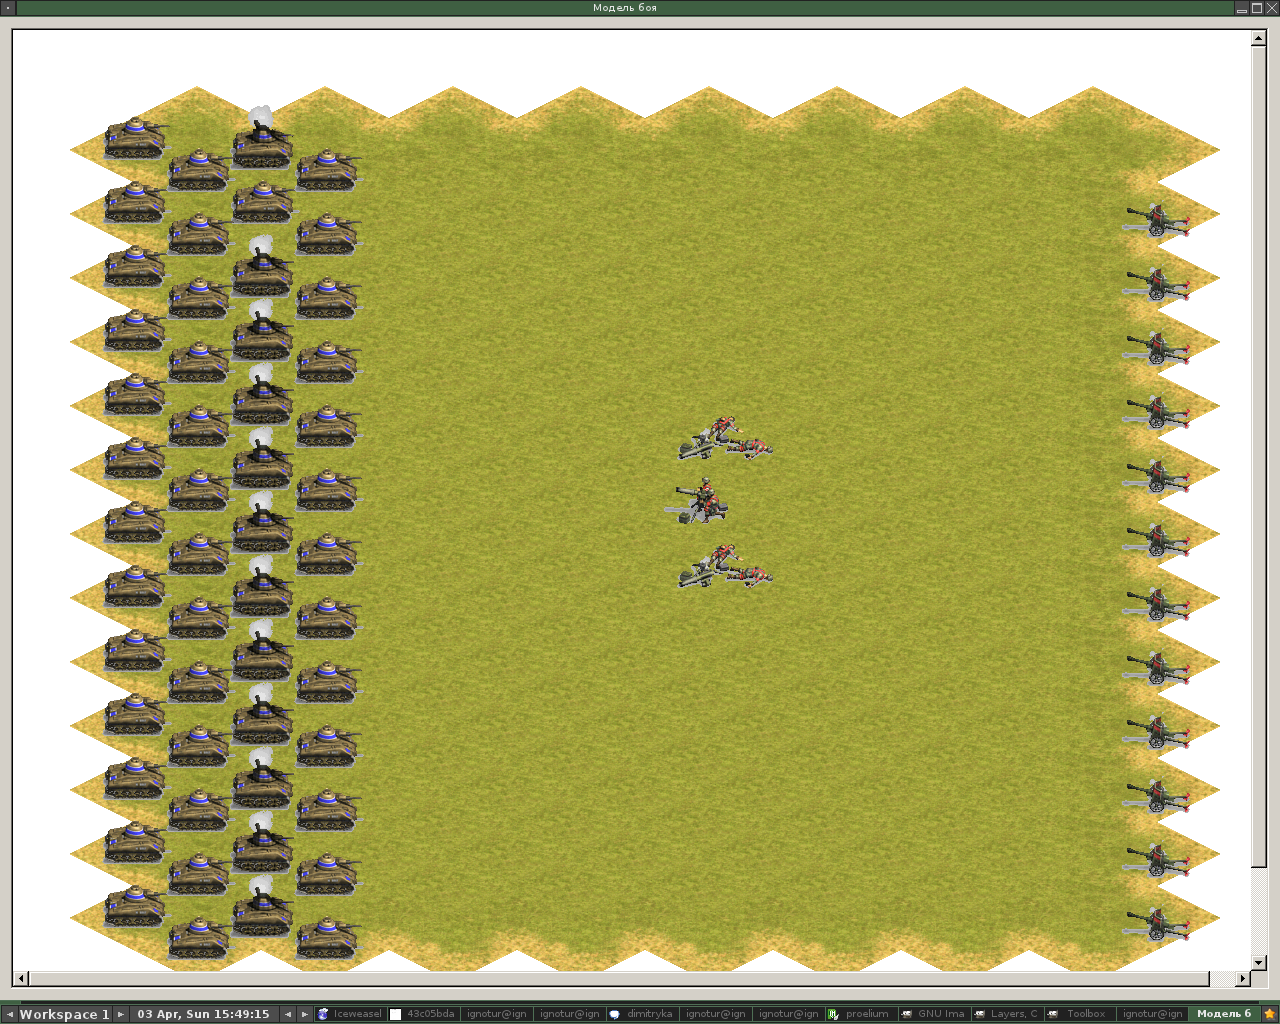
\includegraphics[height=70mm]{img2.png}
\end{center}


\end{document}
